\section{Rozwiązania projektowe}

\subsection {Środowisko}
Obecnie coraz większa część systemów informatycznych realizowana jest w~postaci aplikacji z~dostępem z~poziomu przeglądarki internetowej. Taki zabieg pozwala na~bardzo łatwy dostęp do~systemu z~poziomu praktycznie dowolnego urządzenia posiadającego dostęp do~internetu. Innymi kluczowym czynnikiem jest duża łatwość w~dystrybucji takiego rozwiązania i~w~związku z~tym klient również zdecydował się na~zastosowanie takiego podejścia.\\

Środowiskiem pracy dla użytkowników tworzonego systemu będzie przeglądarka internetowa. Dzięki temu klienci będą mogli korzystać z~dostarczonego systemu zarówno przy użyciu komputera osobistego jak i~urządzenia mobilnego. Rozwiązanie takie jak dedykowane aplikacje mogą być przydatne na~niektórych rodzajach urządzeń, jednak tworzenie ich na~wszystkie możliwe rynki (stacjonarne, mobile itp.) stanowiłoby duże wyzwanie i~spowodowało znaczące przekroczenia zarówno budżetu jak i~harmonogramu.\\

Zdecydowano się na~wsparcie następujących rodzajów przeglądarek:
\begin{enumerate}
  \item Google Chrome (od~wersji 23 wzwyż)
  \item Mozilla Firefox (od~wersji 21 wzwyż)
  \item Safari (od~wersji 6 wzwyż)
  \item Opera (od~wersji 15 wzwyż)
  \item Internet Explorer (od~wersji 10 wzwyż)
\end{enumerate}

Pozostałe przeglądarki także powinny poprawnie prezentować stronę internetową sklepu, jednak wsparcie dla nich nie jest wymaganiem, a~co~za~tym idzie, dla przeglądarek tych nie będą przeprowadzane testy.\\

Wygląd strony internetowej powinien być taki sam (z~różnicami maksymalnie 0.04\% zawartości) dla każdej przeglądarki internetowej. Ewentualne różnice wynikające na przykład z~różnicy w~formatach monitorów czy ich wielkości powinny być obsługiwane przez mechanizmy wewnętrzne.\\

Ewentualne aplikacje wspomagające korzystanie ze~sklepu (na~przykład zdobywające coraz większą popularność aplikacje na~urządzenia mobilne) nie znajdują się w~fazie analizy w~niniejszym projekcie, ewentualnie mogą zostać stworzone w~czasie rozbudowy i~utrzymywania systemu. Aby pozostawić możliwość tego rodzaju rozszerzeń należy zadbać o~odpowiedni protokół komunikacyjny uniezależniający działanie serwerów aplikacyjnych i~bazy danych od~klienta, który dostarcza dane i~polecenia.

\subsection{Architektura}
% TODO Kuba

Jedną z~głównych decyzji w~czasie procesu projektowania tworzonego systemu jest wybór odpowiedniej architektury. Nasza
aplikacja będzie wykorzystywała architekturę trójwarstwową (\textit{ang.} three-tier architecture), ponieważ jest to
najpopularniejsza architektura stosowana w~aplikacjach dostępnych z~poziomu przeglądarki internetowej. Architektura
trójwarstwowa jest przykładem aplikacji typu klient-serwer. Dzieli się ją na trzy warstwy, dzięki czemu proces tworzenia
i nanoszenia poprawek jest łatwiejszy. Co więcej, daje to możliwość zredukowania zależności pomiędzy modułami programu.
Architektura składa się z~następujących warstw: 
\begin{itemize}
  \item \textbf{warstwa danych} (\textit{ang.} data tier)~--~odpowiada za trwałe przechowywanie danych, udostępnia
    interfejs do ich pobierania i~modyfikacji. Realizowana za pomocą relacyjnej bazy danych.
  \item \textbf{warstwa logiki biznesowej} (\textit{ang.} business logic tier)~--~odpowiada za logikę całego systemu,
  koordynuje działania odpowiadające operacjom na kontach i~użytkownikach. Znajduje się na serwerze aplikacyjnym. Pełni
  rolę pośrednika pomiędzy pozostałymi warstwami.
  \item \textbf{warstwa prezentacji} (\textit{ang.} presentation tier)~--~odpowiada za prezentowanie aplikacji na
  komputerze użytkownika, zbieranie jego akcji i~przekazywanie ich do warstwy logiki biznesowej.
\end{itemize}

Wybór architektury trójwarstwowej pociąga za sobą technologie w~jakie zostaną zastosowane. Do stworzenia interfejsu
użytkownika wykorzystane zostaną technologie wykorzystywane w~projektowaniu stron internetowych, czyli HTML i~CSS. Aby
poprawić User Experience, można również założyć wykorzystanie języka JavaScript oraz technologii AJAX. Warstwa logiki,
czyli tzw. backend zostanie stworzony przy użyciu języka Java, ze względu na wydajność, łatwość we wprowadzaniu
zmian, oraz rozbudowaną dokumentację. Dodatkowo wykorzystany zostanie framework webowy SpringMVC. Jako system
zarządzania bazą danych (\textit{ang.} DBMS) postanowiono wykorzystać PostgreSQL.

\begin{figure}[H]
  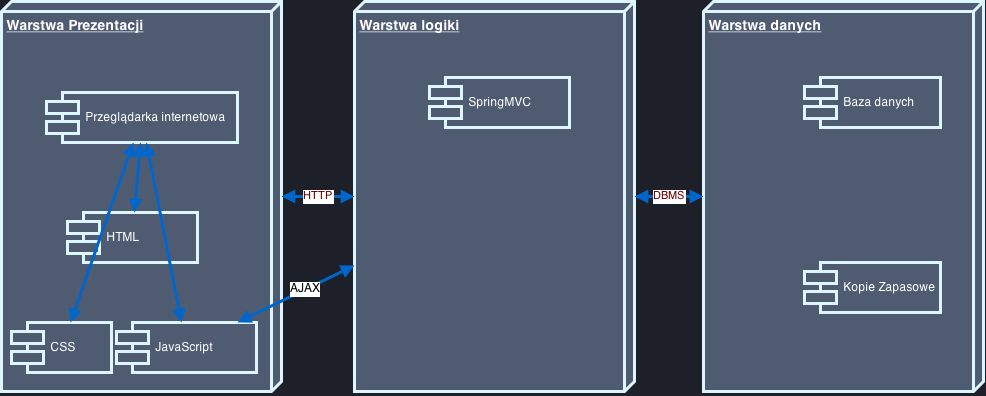
\includegraphics[width=\textwidth]{images/3tier.png}
  \caption{Architektura trójwarstowa, z~zaznaczonymi wybranymi technologiami.}
\end{figure}

\subsection{Sprzęt}

Wdrożenie systemu wymagać będzie zapewnienia odpowiedniej infrastruktury sprzętowej. W celu zapewnienia skalowalności będzie ona podzielona na serwer aplikacyjny i~serwer bazodanowy. Jako że obsługa systemu od strony użytkownika będzie opierać się o~interfejs webowy kompatybilny z!ogromną większością komputerów osobistych wyposażonych w przeglądarkę internetową, wykorzystanie dodatkowych stacji klienckich nie będzie konieczne.

Biorąc pod uwagę takie czynniki jak cena i~wydajność, a~także niezawodność i~głośność pracy, zdecydowano się na wybór komputerów serwerowych z~oferty firmy \textit{Dell}.

\subsubsection{Serwer aplikacyjny}

Jako serwer obsługujący warstwę logiki wybrano \textit{Dell PowerEdge R220} ze względu na korzystny stosunek wydajności do ceny.

\begin{figure}[H]
  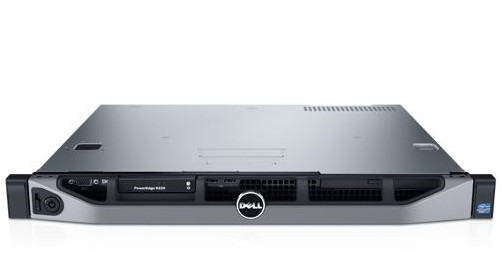
\includegraphics[width=\textwidth]{images/poweredge-r220.jpg}
  \caption{Dell PowerEdge R220}
\end{figure}

\begin{figure}[H]
\begin{center}
\begin{tabular}{|l|l|}
  \hline
  Procesor & Intel® Celeron® G1820 2.7GHz \\ \hline
  Pamięć RAM & 4 x 4GB UDIMM, 1600 MT/s, Low Volt, Single Rank, x8 Data Width \\ \hline
  Dysk & 500GB 7.2k RPM SATA 6Gbps Entry 3.5in Cabled Hard Drive \\ \hline
  Zasilanie & 250W (80+ Silver); auto-ranging (100V--240V) \\ \hline

\end{tabular}
\end{center}
\end{figure}

\subsubsection{Serwer bazy danych}

Baza danych obsługiwana będzie przez serwer \textit{Dell PowerEdge R320}.

\begin{figure}[H]
  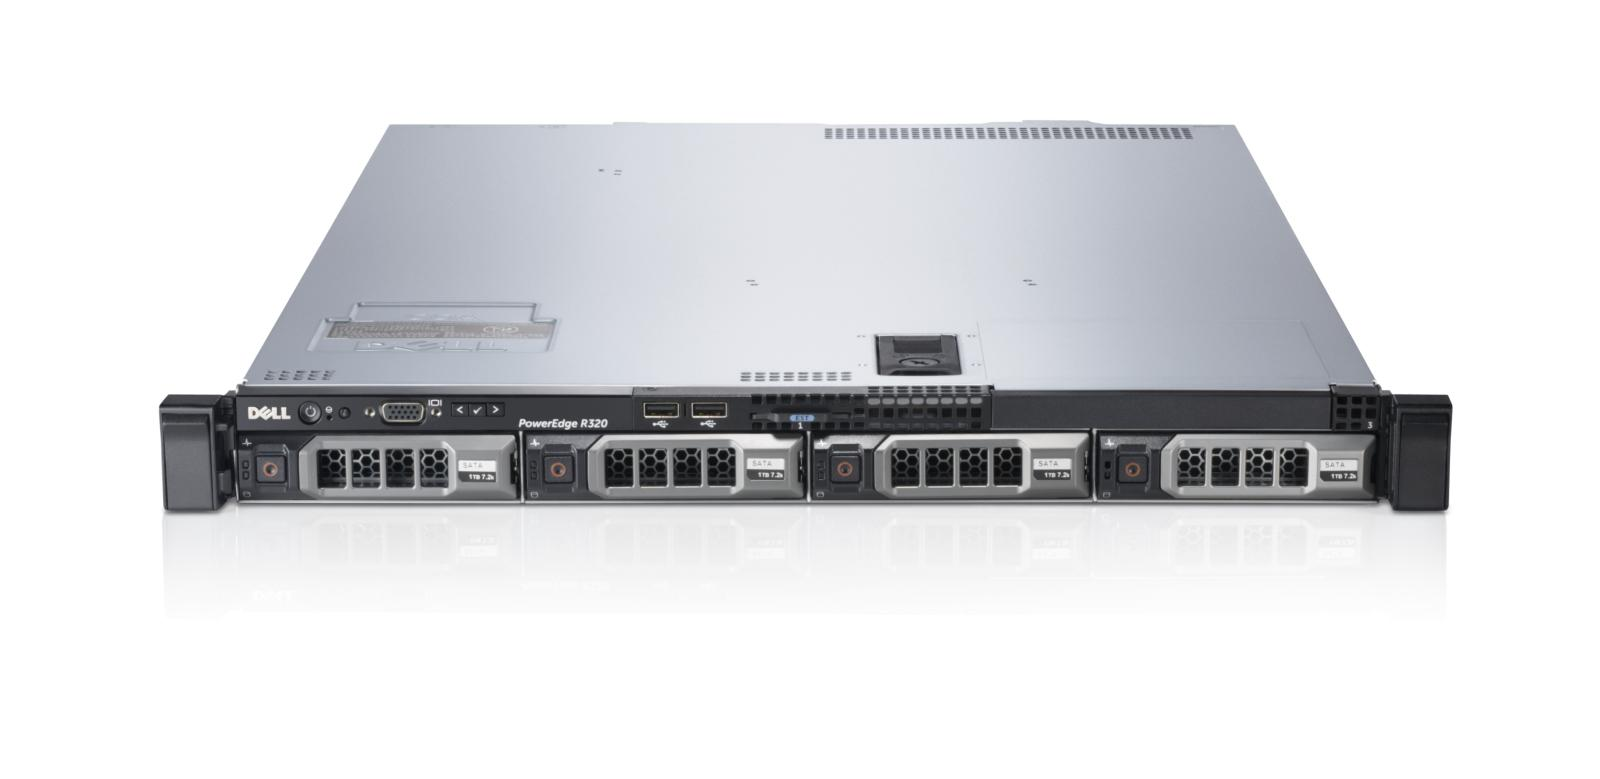
\includegraphics[width=\textwidth]{images/poweredge-r320.jpg}
  \caption{Dell PowerEdge R320}
\end{figure}

\begin{figure}[H]
\begin{center}
\begin{tabular}{|l|l|}
  \hline
  Procesor & Intel® Pentium® 1403 v2 2.60GHz \\ \hline
  Pamięć RAM & 4 x 4GB UDIMM, 1600 MT/s, Low Volt, Single Rank, x8 Data Width \\ \hline
  Dysk & 500GB 7.2k RPM SATA 6Gbps Entry 3.5in Cabled Hard Drive \\ \hline
  Zasilanie & 350W (80+ Silver); auto-ranging (100V--240V) \\ \hline

\end{tabular}
\end{center}
\end{figure}

\subsubsection{Szafa rack}

Oba serwery wyposażone są w obudowy typu \textit{rack 19''} i~są kompatybilne z~wszelkiego rodzaju szafami wykorzystującymi ten standard. Biorąc pod uwagę niewielkie rozmiary i solidność wykonania, sugerowane jest wykorzystanie szafy serwerowej \textit{Signati 12U}.

\begin{figure}[H]
  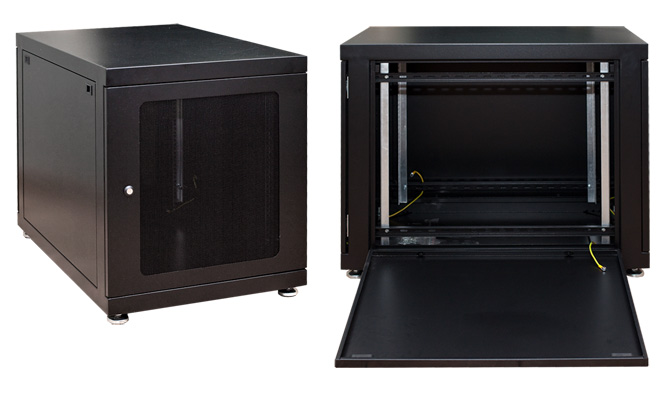
\includegraphics[width=\textwidth]{images/szafa_12U.jpg}
  \caption{Signati 12U}
\end{figure}